\documentclass{beamer}

\usepackage{cmap}				% To be able to copy-paste russian text from pdf
\usepackage[T2A]{fontenc}
\usepackage[utf8]{inputenc}
\usepackage[english]{babel}
\usepackage{textpos}
\usepackage{ragged2e}
\usepackage{amssymb}
\usepackage{ulem}
\usepackage{tikz}
\usepackage{pgfplots}
\usepackage{color}
\usepackage{cancel}
\usepackage{multirow}
\pgfplotsset{compat=1.17}
\usetikzlibrary{arrows,snakes,backgrounds,shapes}
\usepgfplotslibrary{groupplots,colorbrewer,dateplot,statistics}
\usepackage{animate}

\usepackage{amsfonts}
\usepackage{amsmath}
\usepackage{amssymb}
\usepackage{graphicx}
\usepackage{setspace}
\usepackage{tabularx}

\usepackage{enumitem}
	\setitemize{label=\usebeamerfont*{itemize item}%
	  \usebeamercolor[fg]{itemize item}
	  \usebeamertemplate{itemize item}}
	

\usepackage{eurosym}
\renewcommand{\EUR}[1]{\textup{\euro}#1}

\title{Credit Default Swaps}
\author{Artem Bakulin}
\date{November 19, 2024}


	\usetheme{Warsaw}
	\usecolortheme{beaver}

	\newcommand{\inserttitleframe}{
		\begin{frame}
		\titlepage
		\end{frame}
	}
	
	\newcommand{\insertdisclaimerframe}{
	}
	
	% remove navigation bar
	\setbeamertemplate{navigation symbols}{}

	% add page counter
	\setbeamertemplate{page number in head/foot}[totalframenumber] 

	% remove navigation bar
	\setbeamertemplate{navigation symbols}{}
	
	\setbeamertemplate{page number in head/foot}[totalframenumber] 


\newcommand{\ru}[1]{\begin{otherlanguage}{russian}#1\end{otherlanguage}}
\newcommand{\en}[1]{\begin{otherlanguage}{english}#1\end{otherlanguage}}
\newcommand{\ruen}[2]{#1 (\en{#2})}

% https://tex.stackexchange.com/questions/98003/filter-rows-from-a-table
\pgfplotsset{
    discard if not/.style 2 args={
        x filter/.code={
            \edef\tempa{\thisrow{#1}}
            \edef\tempb{#2}
            \ifx\tempa\tempb
            \else
                \def\pgfmathresult{inf}
            \fi
        }
    }
}



\begin{document}

\inserttitleframe

\begin{frame}{Reminder: bonds}
\justify
A \alert{bond} is a debt security that entitles the holder (the lender) to receive pre-determined cash flows (interest coupons and principal amount) from the issuer (the borrower).

\justify
\alert{Yield to maturity (YTM)} is the discount rate at which total present value of all the bond's future cash flows is equal to the current market price of this bond.

\justify
Consider a 3-year bond that pays 5\% coupon annually and has a principal amount (i.e. face value) of \$1\,000. Its current market price is \$980 (98\% of the face value).
\begin{equation*}
\$980 = \frac{\$50}{1+y} + \frac{\$50}{(1+y)^2} + \frac{\$1\,000 + \$50}{(1+y)^3}  \quad  \Leftrightarrow \quad y \approx 5.745\%
\end{equation*}

\justify
Lower the market price of a bond, higher the yield to maturity. Yields are just a more convenient way of measuring the same observable reality and comparing different bonds.
\end{frame}



\begin{frame}{Reminder: credit spread}
\justify
\alert{Credit spread} is a difference between yields of a corporate bond and a comparable government bond (assuming matching maturity and currency).
\begin{align*}
CreditSpread &= CorpYield - GovtYield \\
 CorpYield &= GovtYield + CreditSpread
\end{align*}

\justify
Suppose you invest in a corporate bond. You lose money in case the bond price falls and the bond yield rises. The bond yield may raise due to two reasons:

1. Increase in the government bond yield due to general macro-economic reasons (e.g. inflation, central bank policy).

2. Widening of the credit spread due to issuer-specific reasons (e.g. poor production results).

\justify
Can we decouple our results from the uncontrollable generic macro-economic factors? 
\end{frame}



\begin{frame}{Credit default swap}
\justify
A \alert{credit default swap (CDS)} is a financial derivative that allows buying or selling insurance against default on bonds or other debts.

\justify
Key parameters of a swap:

\justify
1. Reference entity: the entity whose default is covered by the insurance. E.g. FooBar LLC. It is neither buyer nor seller of the swap, it does not take part in the contract

\justify
2. Notional amount or insured amount. E.g. \$10\,000\,000.

\justify
3, Coverage period. E.g. starting today and ending in a year.

\justify
4, Fixed coupon (spread): percentage of the notional amount which the buyer pays to the seller. E.g. 2\% annually.

\justify
Buying a CDS means agreeing to pay fixed coupons in exchange for insurance. 
\end{frame}



\newcommand{\swapPartyNode}[5]{

	\draw (#1, #2)
		node[
			rectangle,
			draw,
			rounded corners,
			anchor = south,
			minimum height = 0.8cm,
			minimum width = 2.5cm
		]
		{#5}
	--
	(#3, #4);
}

\newcommand{\swapBuyerPaymentEx}[7]{

	\draw [
		->,
		>=triangle 90
	] 
	(#1, #2)
	node[
		label = left:{#7}
	]{}
	-- (#3, #4)
	node[
		pos=0.5,
		anchor=south
	]
	{#5}
	node[
		pos=0.5,
		anchor=north
	]
	{#6};
}

\newcommand{\swapBuyerPayment}[6]{

	\swapBuyerPaymentEx{#1}{#2}{#3}{#4}{#5}{}{#6}
}

\begin{frame}{Credit default swap - 2}
\justify
CDS term is 1 year, notional amount is \$10\,000\,000, coupon is $2.0\%$.

\justify
\centering
\begin{tikzpicture}[thick]

		\swapPartyNode{0}{0}{0}{-4}{Buyer}
		
		\swapPartyNode{5.5}{0}{5.5}{-4}{Seller}
		
		\swapBuyerPayment{0}{-1}{2.5}{-1}{\$50\,000}{3 months}
		\swapBuyerPayment{0}{-2}{2.5}{-2}{\$50\,000}{6 months}
		\swapBuyerPayment{0}{-3}{2.5}{-3}{\$50\,000}{9 months}
		\swapBuyerPayment{0}{-4}{2.5}{-4}{\$50\,000}{12 months}
\end{tikzpicture}
\end{frame}



\begin{frame}{Credit default swaps - 3}
\justify
The reference entity announced bankruptcy in 8 months.

\justify
\centering
\begin{tikzpicture}[thick]
		\swapPartyNode{0}{0}{0}{-2.67}{Buyer}
		
		\swapPartyNode{5.5}{0}{5.5}{-2.67}{Seller}
		
		\swapBuyerPayment{0}{-1}{2.5}{-1}{\$50\,000}{3 months}
		\swapBuyerPayment{0}{-2}{2.5}{-2}{\$50\,000}{6 months}
		\swapBuyerPaymentEx{0}{-2.67}{2.5}{-2.67}{\$33\,000}{Bond}{8 months}
		
		\swapBuyerPayment{5.5}{-2.67}{3}{-2.67}{\$10\,000\,000}{}
\end{tikzpicture}
\end{frame}



\begin{frame}{Deliverable and cash-settled swaps}
\justify
Suppose that a default has happened

1. Insured notional amount \$10\,000\,000.

2. Market price of the defaulted bond is \$4\,000\,000.

\justify
\alert{Deliverable} credit default swap:

1. The buyer hands over defaulted bonds to the seller.

2. The seller pays the buyer full notional amount (\$10\,000\,000).

\justify
\alert{Cash-settled} credit default swap:

1. The seller pays the buyer the difference between notional amount and market value of the bonds  (\$6\,000\,000).

\end{frame}



\begin{frame}{Hedging credit risk}
\justify
Suppose we own a corporate bond. Negative news has been announced, and now we are concerned that the probability of default has increased. We have two options:

1. Sell the bond on the market.

2. Buy insurance, i.e. buy a credit default swap.

\justify
In theory, if there was an ideal perfectly liquid market for bonds, we would sell the bond immediately at zero bid/ask spread. In practice, it may take weeks to find a buyer for an illiquid security..

\justify
Sometimes buying a credit default swap may be simpler and more cost-effective than selling an illiquid bond. When (and if) the market stabilizes we sill sell the swap.

\justify
Credit default swaps are particularly useful for hedging non-traded debts, such as bank loans.
\end{frame}



\begin{frame}{Speculating on credit risk}

\justify
We have a view that creditworthiness of a reference entity will deteriorate in future. Our options are:

1. Sell short the risky bond and buy a risk-free government bond (to eliminate the general interest rate risk).

2. Buy a credit default swap.

\justify
Do you have to own a bond  to buy a CDS? No! This position would be called a naked CDS (*).

\justify
A small bank could be selling credit default swaps to diversify its credit portfolio. It could "make loans"\ to companies (reference entities) that would never speak to this bank otherwise.

\justify
(*) The EU regulation prohibits naked CDS in case reference entity is one of the EU governments.
\end{frame}


\renewcommand{\swapPartyNode}[4]{

	\draw (#1, #2)
		node[
			rectangle,
			draw,
			rounded corners,
			anchor = south,
			minimum height = 0.8cm,
			minimum width = 2.8cm
		]
		(#4)
		{#3};
}

\newcommand{\paymentFlow}[4] {
	\draw [
		->,
		>=triangle 90
	]
	(#1) -- (#2)
	node[
		pos = 0.5,
		anchor = #4
	]
	{#3};
}

\begin{frame}{Speculating on credit risk - 2}
\justify
We have bought a swap from company A at 2\%, and managed to a sell similar swap to company B at 3\%. We will be making 1\% of the notional amount per annum until the default happens or until maturity of the swaps.

\justify
\centering
\begin{tikzpicture}

	\swapPartyNode{0}{2}{Company A}{A}
	\swapPartyNode{0}{0}{Speculator}{S}
	\swapPartyNode{0}{-2}{Company B}{B}
	
	\paymentFlow{[xshift=-0.5cm] S.north}{[xshift=-0.5cm] A.south}{2\%}{east};
	\paymentFlow{[xshift=-0.5cm] B.north}{[xshift=-0.5cm] S.south}{3\%}{east};
	
	\paymentFlow{[xshift=+0.5cm] A.south}{[xshift=+0.5cm] S.north}{Insurance}{west};
	\paymentFlow{[xshift=+0.5cm] S.south}{[xshift=+0.5cm] B.north}{Insurance}{west};
	
	\swapPartyNode{6}{2}{Company А}{A}
	\swapPartyNode{6}{0}{Speculator}{S}
	\swapPartyNode{6}{-2}{Company B}{B}
	
	\paymentFlow{[xshift=-0.5cm] A.south}{[xshift=-0.5cm] S.north}{Notional amount}{east};
	\paymentFlow{[xshift=-0.5cm] S.south}{[xshift=-0.5cm] B.north}{Notional amount}{east};
	
	\paymentFlow{[xshift=+0.5cm] S.north}{[xshift=+0.5cm] A.south}{Bond}{west};
	\paymentFlow{[xshift=+0.5cm] B.north}{[xshift=+0.5cm] S.south}{Bond}{west};
\end{tikzpicture}
\end{frame}



\begin{frame}{Speculating on credit risk - 3}
\justify
We have a view that creditworthiness of a reference entity will improve in future. We have two options: 

\justify
1. Buy the risky bond and sell short a risk-free government bond (to eliminate the general interest rate risk).

\justify
2. Sell a credit default swap.

\justify
If we sold a swap to company A at 3\%, and bought s similar swap from company B at 2\%, then we will be making 1\% per annum until a default happens or until maturity of the swaps.
\end{frame}



\begin{frame}{Factors affecting a CDS price}
\justify
A few factors affect fair price of a CDS.

\justify
1. Probability of default. It can be estimated from other CDS quotes or from market prices for this entity's bonds.

\justify
2. Recovery rate is residual value of a bond in case of default. Usually it is estimated from historical data for particular jurisdiction, economy sector, credit rating.

\justify
3. Discounting interest rate for future cash flows.
\end{frame}



\begin{frame}{Recovery rate}
\justify
Moody's Corporate Default and Recovery Rates, 1920--2010.

\vspace{\baselineskip}
\begin{tabular}{l|l|l|l}
Position						& 2010		& 2009		& 1982--2010 \\
\hline
1st	Lien Bank Loan	 		& 72.30\%	& 56.30\% & 59.60\% \\
2nd Lien Bank Loan 		& 18.40\%	& 20.80\% & 27.90\% \\
Sr. Unsecured	Bank Loan	& n.a.		& 37.90\% & 39.90\% \\
Sr. Secured Bond			& 54.70\%	& 29.60\% & 49.10\%	 \\
\hline
Sr. Unsecured	Bond		& 63.80\%	& 35.50\% & 37.40\%	 \\
\hline
Sr. Subordinated Bond	& 39.40\%	& 18.00\% & 25.30\%	\\
Subordinated Bond		& 32.20\%	& 25.10\% & 24.20\%	\\
Jr. Subordinated Bond	 	& n.a.		& n.a.		&17.10\%	\\
\end{tabular}

\justify
Rule of thumb: 40\%.
\end{frame}



\begin{frame}{Credit rating}
\justify
Why don't we check credit rating to estimate probability of default? This is Standard \& Poor's scale (best to worst):
\begin{align*}
\text{Investment-grade}
\small
&\begin{cases}
\small \text{AAA} \\
\small \text{AA+, AA, AA-} \\
\small \text{A+, A, A-} \\
\small \text{BBB+, BBB, BBB-,}
\end{cases} \\
\text{Speculative-grade}
&\begin{cases}
\small \text{BB+, BB, BB-,} \\
\small \text{B+, B, B-,} \\
\small \text{CCC+, CCC, CCC-,} \\
\small \text{CC,C, D}
\end{cases}
\end{align*}
\end{frame}



\newcommand{\addDefaultRatePlot}[3] {

	\addplot[
		color = #2,
		mark = #3,
		thick
	]
	table[
		x = year,
		y = #1,
		col sep = comma
	]
	{sp_2020_global_corporate_default_rates.csv};
}

\begin{frame}{Credit-rating - 2}
\justify
Ratings reflect relative riskiness rather than absolute probability.

\justify
\centering
\begin{tikzpicture}
	\begin{axis}[
		width = \textwidth,
		height = \textheight - 1.5cm,
		ymin = 0,
		ymax = 13,
		xmin = 1981,
		xmax = 2024,
		grid = major,
		xticklabel = {\pgfmathprintnumber[precision=0, 1000 sep=]{\tick}},
		yticklabel = {\pgfmathprintnumber[precision=0]{\tick}\%},
		ylabel = {Default frequency},
		legend entries = {
  	   		\small Speculative-grade,
      		\small Investment-grade
  		},
  		legend cell align={left}
	]
		
		\addDefaultRatePlot{speculative_grade_default_rate}{Set1-A}{square}
		
		\addDefaultRatePlot{investment_grade_default_rate}{Set1-B}{*}
	\end{axis}
\end{tikzpicture}

\centering
\small Data: \en{S\&P Global}
\end{frame}



\begin{frame}{Bond price and probability of default}
\justify
A risk-free zero-coupon government bond that matures in 1 year is priced at $G=98\%$ of its face value. If you invest \$980 today you receive \$1\,000 in a year. Rate of return is $\$1\,000 / \$980 - 1 \approx 2.04\%$.

\justify
A corporate bond of the same maturity is priced at $C=95\%$ of its face value. If you invest \$950 today, you receive \$1\,000 in a year (in case there is no default). Rate of return is $\$1\,000 / \$950 - 1 \approx 5.3\%$.

\justify
Why do market participants value the corporate bond less, i.e. demand higher rate of return?

\justify
Suppose that the recovery rate in case of default is $R=40\%$. You invest \$950 today and receive \$400 in a year. Rate of return in case of default is $\$400 / \$950 - 1 = -57.9\%$.
\end{frame}



\begin{frame}{Bond price and probability of default - 2}
\justify
Government bond is worth $G=98\%$ of its face value, corporate bond is worth $C=95\%$, recovery rate in case of default is $R=40\%$.

\justify
Which default probability $p$ equalizes two expected rates of return?

\justify
\centering
\begin{tabular}{l|c|c|c|c|c}
& & \multicolumn{2}{c|}{Default ($p$)} & \multicolumn{2}{c}{No default ($1-p$)} \\
Bond & Price & Payoff & Return & Payoff & Return \\
\hline
Govt.  & 0.98 & 1     & 1/0.98 - 1 & 1 & 1/0.98 - 1\\
Corp. & 0.95 & 0.4 & 0.4/0.95 - 1 & 1 & 1/0.95 - 1
\end{tabular}

\justify
Expected rates of return should be equal:
\begin{align*}
\frac{1}{0.98} - 1 &= p\left(\frac{0.4}{0.95} - 1\right) + (1-p)\left(\frac{1}{0.95} - 1\right) \Rightarrow \\
p &= \frac{1 - C/G}{1-R} = \frac{1 - 0.95/0.98}{1-0.4} \approx 5.1\%
\end{align*}
\end{frame}



\begin{frame}{Bond price and probability of default - 3}
\justify
We can re-write the formula in terms of bond yields $r_g$ и $r_c$. Suppose that two bonds mature in $T$ years.
\begin{align*}
G = \frac{1}{(1 + r_g)^T}, C = \frac{1}{(1 + r_c)^T}
\end{align*}
Then
\begin{align*}
p = \frac{1 - \dfrac{C}{G}}{1-R} = \frac{1 - \dfrac{(1 + r_g)^T}{(1 + r_c)^T}}{1 - R}
\end{align*}

\justify
(We assume that in case of default we will recover the residual value on maturity date)
\end{frame}



\begin{frame}{Probability of default and credit spread}
\justify
In case interest rates are not too high, we can simplify the formula:
\begin{equation*}
p = \frac{1 - \dfrac{(1 + r_g)^T}{(1 + r_c)^T}}{1 - R} \approx \frac{T(r_c - r_g)}{1 - R}
\end{equation*}

\justify
For example, a one-year bond of a large German Frankfurt-based investment bank yields 3.7\%. Similar German government bond yields $2.4\%$. Recovery rate in case of bankruptcy is 40\%.

\justify
What is probability that the bank will default during a year?
\begin{equation*}
p \approx \frac{r_{Bank} - r_{Germany}}{1-R} = \frac{3.7\% - 2.4\%}{1-40\%} \approx 2.17\%
\end{equation*}
\end{frame}



\begin{frame}{Interpolating the probability of default}
\centering
\begin{tabular}{l|r|r|r|r}
Term & Govt. Yield & Corp. Yield & Recovery & PD \\ \hline
1Y & 1.00\% & 2.23\% & 40\% & 2.00\% \\
2Y & 1.50\% & 3.06\% & 40\% & 5.00\%
\end{tabular}

\justify
What is probability of the default happening between now and $T^*=1.5$ years from now?

\justify
Suppose that $\xi$ is a random variable that denotes the time till default in years.

\justify
$D(T)$ is probability that the default will happen until time $T$. $S(T)$ is probability that the reference entity will survive till time $T$.
\begin{align*}
D(T) &= \mathbb{P}(\xi < T) \\
S(T) &= \mathbb{P}(\xi \ge T) = 1 - D(T)
\end{align*}
\end{frame}
 


\begin{frame}{Reminder: geometric distribution}
\justify
Suppose we are flipping a coin. Probability of Tails outcome is $p$ (usually it is close to 50\%). We continue flipping the coin until the first Tails outcome (a default). We are interested in a random variable $\xi$ which is the number or Heads until the first Tails (years without a default).

\justify
What is probability that the first Tail will occur not sooner than in the $n$-th trial (i.e. we get at least $n$ Heads in a row)?
\begin{align*}
\mathbb{P}(\xi \ge n) = S(n) = (1 - p)^{n}
\end{align*}
\justify
$\xi$ is said to follow geometric distribution.
\end{frame}



\begin{frame}{Reminder: geometric distribution - 2}
\centering
\begin{tikzpicture}
\begin{axis}[
    width = \textwidth,
    height = \textheight - 1cm,
    xmin = 0, xmax = 10,
    ymin = 0, ymax = 1,
    xtick distance=1,
    ytick distance=0.1,
    grid=major
]

\addplot[color=Set1-A, thick, mark=*, domain=0:10, samples=11]{(1-0.5)^x)};
\end{axis}
\end{tikzpicture}
\end{frame}



\begin{frame}{Reminder: exponential distribution}
\justify
Suppose that the default may happen at any time, not just once a year. Suppose that during any tiny time interval $dt$ a default may happen with probability of $\lambda \cdot dt$. $\lambda$ is called \alert{hazard rate} and it is usually expressed in percent per annum.

\justify
Probability that a reference entity survives till time $T$ is $S(T)$. What is probability that it will survive a bit longer?
\begin{align*}
S(T+dt) = S(T)(1 - \lambda dt)
\end{align*}

\justify
Rearranging the terms and solving a tiny differential equation:
\begin{align*}
\frac{S(T+dt) - S(T)}{dt} = -\lambda S(T) \quad
\Rightarrow
\quad
S(T) = e^{-\lambda T}
\end{align*}
\justify
This is an exponential distribution, a continuous version of discrete geometric distribution.
\end{frame}



\begin{frame}{Reminder: exponential distribution - 2}
\centering
\begin{tikzpicture}
\begin{axis}[
    width = \textwidth,
    height = \textheight - 1cm,
    xmin = 0, xmax = 10,
    ymin = 0, ymax = 1,
    xtick distance=1,
    ytick distance=0.1,
    grid=major
]

\addplot[color=Set1-A, thick, domain=0:10]{exp(-x*ln(2))};
\end{axis}
\end{tikzpicture}
\end{frame}



\begin{frame}{Interpolating the probability of default - 2}
\centering
\begin{tabular}{l|r|r|r|r}
Term & Govt. Yield & Corp. Yield & Recovery & PD \\ \hline
1Y & 1.00\% & 2.23\% & 40\% & 2.00\% \\
2Y & 1.50\% & 3.06\% & 40\% & 5.00\%
\end{tabular}

\justify
What is probability of the default happening between now and $T^*=1.5$ years from now?

\justify
Suppose that after surviving through $T_1=1$ year, the reference entity finds itself under hazard rate $\lambda$ in an exponential distribution.

\justify
Formally, for any $T^*$ between $T_1=1$ and $T_2=2$ years it holds that
\begin{align*}
S(T^*) = S(T_1)e^{-\lambda(T^* - T_1)}
\end{align*}
\end{frame}





\newcommand{\nodeWithDropLines}[2]{
    \node[
        circle,
        fill,
        color=Set1-A,
        inner sep=2pt
    ]
    at (axis cs: #1, #2)
    {};

    \draw[
        dashed,
        thick
    ]
    (axis cs: 0, #2) -- (axis cs: #1, #2) -- (axis cs: #1, 0);
}

\begin{frame}{Interpolating the probability of default - 3}
\centering
\begin{tikzpicture}
\begin{axis}[
    width = \textwidth,
    height = \textheight - 1cm,
    xmin = 0, xmax = 3,
    ymin = 0, ymax = 1.2,
    xtick = {1, 2},
    xticklabels = {$T_1$, $T_2$},
    xtick pos = left,
    ytick = {0.404, 0.9, 1},
    yticklabels = {$S(T_2)$, $S(T_1)$, 1},
    ytick pos = left,
    axis lines = middle
]

\addplot[color=Set1-A, thick, domain=0:1]{exp(ln(0.9)*x)};
\addplot[color=Set1-A, thick, domain=1:2]{0.9 * exp(-0.8 * (x - 1))};
\addplot[color=Set1-A, thick, domain=2:3]{0.9*exp(-0.8)*exp(-2*(x-2))};

\nodeWithDropLines{1}{0.9}
\nodeWithDropLines{2}{0.404}

\node[anchor=west] at (axis cs: 1.5, 0.65) {$S(T_1)e^{-\lambda (T - T_1)}$};

\end{axis}
\end{tikzpicture}
\end{frame}




\begin{frame}{Interpolating the probability of default - 4}
\justify
We can derive the value of $\lambda$ from $S(T_1)$ and $S(T_2)$.
\begin{align*}
S(T_2) = S(T_1)e^{-\lambda(T_2-T_1)}
\end{align*}
Consequently
\begin{align*}
\lambda = \dfrac{\ln\left(\dfrac{S(T_1)}{S(T_2)}\right)}{T_2 - T_1} = \dfrac{\ln\left(\dfrac{1 - D(T_1)}{1 - D(T_2)}\right)}{T_2 - T_1}
\end{align*}
In our particular case, $\lambda \approx 3.11\%$. So we can interpolate the value of $D(1.5)$:
\begin{align*}
D(1.5) = 1 - S(1.5) = 1 - (1 - D(1))e^{-3.11\% \cdot (1.5 - 1)} \approx 3.51\%
\end{align*}
\end{frame}



\begin{frame}{Pricing a credit default swap}
\justify
Suppose that we know the probability of default, recovery rate, and discount factors for future cashflows. How to we compute fair coupon in a credit default swap?

\justify
Expected discounted cashflows of the buyer and the seller should match.

\justify
We compute two values for each future date:

\justify
1. Probability of the reference entity surviving till this date, $S(T)$.

\justify
2.Probability of the reference entity defaulting precisely on this day, $D(T) - D(T - 1 \text{ day})$.
\end{frame}



\begin{frame}{Pricing a credit default swap - 2}
\justify
With probability $S(T)$, the buyer pays a coupon in case $T$  is one of the coupon dates.
\begin{center}
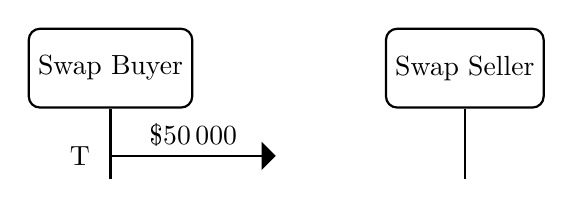
\begin{tikzpicture}[thick, scale=0.6]
		\draw (0, 0) node[rectangle,draw,rounded corners,anchor=south,minimum height=1cm] {Swap Buyer} -- (0, -1.5);
		\draw (7.5, 0) node[rectangle,draw,rounded corners,anchor=south,minimum height=1cm] {Swap Seller} -- (7.5, -1.5);
		\draw [->,>=triangle 90] (0, -1.0) node[label=left:{T}]{} -- (3.5, -1.0) node[pos=0.5,anchor=south]{\$50\,000};
\end{tikzpicture}
\end{center}

\justify
With probability $D(T) - D(T - 1 \text{day})$, the buyer pays the accrued interest and delivers the defaulted bond, the seller pays out the swap notional amount.
\begin{center}
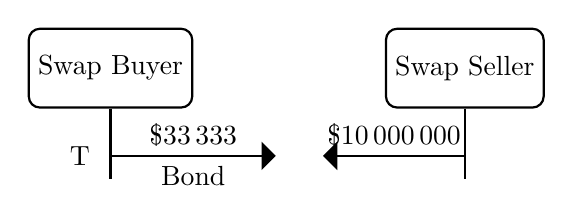
\begin{tikzpicture}[thick, scale=0.6]
		\draw (0, 0) node[rectangle,draw,rounded corners,anchor=south,minimum height=1cm] {Swap Buyer} -- (0, -1.5);
		\draw (7.5, 0) node[rectangle,draw,rounded corners,anchor=south,minimum height=1cm] {Swap Seller} -- (7.5, -1.5);
		\draw [->,>=triangle 90] (0, -1.0) node[label=left:{T}]{} -- (3.5, -1.0) node[pos=0.5,anchor=south]{\$33\,333} node[pos=0.5,anchor=north] {Bond};
		\draw [->,>=triangle 90] (7.5, -1.0) -- (4.5, -1.0) node[pos=0.5,anchor=south]{\$10\,000\,000};
\end{tikzpicture}
\end{center}
\end{frame}



\begin{frame}{Sample problem}
\justify
Find fair price (coupon) for a credit default swap under following assumptions.

\justify
1. Term is 1 year.

\justify
2.Quarterly coupons (every 1/4th of a year).

\justify
3. Recovery rate is 40\%.

\justify
4. Probability of default is given by a exponential distribution with hazard rate of $\lambda = 2\%$.

\justify
5. In case of a default, the notional amount will be paid on the following coupon date. The swap is cash-settled.

\justify
6. Neglect the discounting.
\end{frame}



\begin{frame}{Solution}
\justify
Let $x$ be an annual coupon rate. Swap notional is $\$1$, recovery rate is $R$. Let $S(t)$ be probability of the reference entity surviving for $t$ years. Write down all payments of the seller and the buyer, along with probabilities of these payments.

\begin{center}
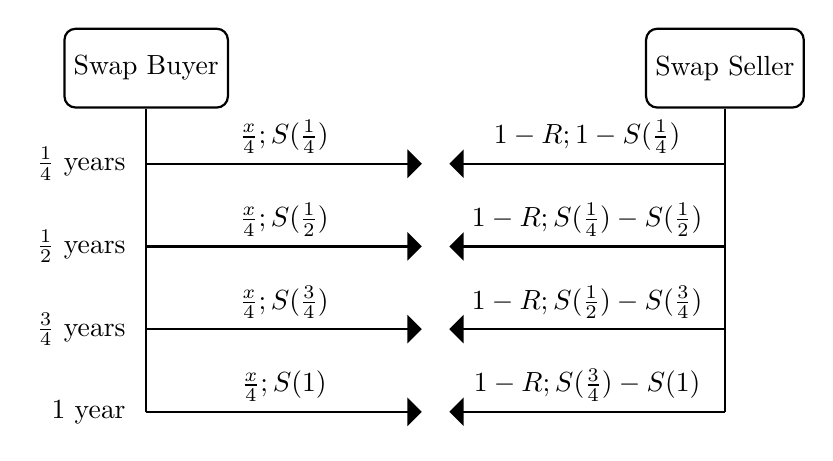
\begin{tikzpicture}[thick, scale=0.7]
		\draw (0, 0) node[rectangle,draw,rounded corners,anchor=south,minimum height=1cm] {Swap Buyer} -- (0, -5.5);
		\draw (10.5, 0) node[rectangle,draw,rounded corners,anchor=south,minimum height=1cm] {Swap Seller} -- (10.5, -5.5);
		\draw [->,>=triangle 90] (0, -1.0) node[label=left:{$\frac{1}{4}$ years}]{} -- (5.0, -1.0) node[pos=0.5,anchor=south]{$\frac{x}{4}; S(\frac{1}{4})$};
		\draw [->,>=triangle 90] (0, -2.5) node[label=left:{$\frac{1}{2}$ years}]{} -- (5.0, -2.5) node[pos=0.5,anchor=south]{$\frac{x}{4}; S(\frac{1}{2})$};
		\draw [->,>=triangle 90] (0, -4.0) node[label=left:{$\frac{3}{4}$ years}]{} -- (5.0, -4.0) node[pos=0.5,anchor=south]{$\frac{x}{4}; S(\frac{3}{4})$};
		\draw [->,>=triangle 90] (0, -5.5) node[label=left:{$1$ year}]{} -- (5.0, -5.5) node[pos=0.5,anchor=south]{$\frac{x}{4}; S(1)$};
    
    \draw [->,>=triangle 90] (10.5, -1.0) -- (5.5, -1.0) node[pos=0.5,anchor=south]{$1-R; 1 - S(\frac{1}{4})$};
    \draw [->,>=triangle 90] (10.5, -2.5) -- (5.5, -2.5) node[pos=0.5,anchor=south]{$1-R; S(\frac{1}{4}) - S(\frac{1}{2})$};
    \draw [->,>=triangle 90] (10.5, -4.0) -- (5.5, -4.0) node[pos=0.5,anchor=south]{$1-R; S(\frac{1}{2}) - S(\frac{3}{4})$};
    \draw [->,>=triangle 90] (10.5, -5.5) -- (5.5, -5.5) node[pos=0.5,anchor=south]{$1-R; S(\frac{3}{4}) - S(1)$};

\end{tikzpicture}
\end{center}
\end{frame}



\begin{frame}{Solution - 2}
\justify
Probability of the reference entity surviving during 1/4 of a year is $S(1/4) = 98\%$. Probability of the reference entity surviving during 1/2 of a year is $S(1/2) = 95\%$. 

\justify
What is probability that the reference entity will default at any time between 1/4 and 1/2 (during the second quarter)? 

\justify
Consider a sample of 100\,000 entities that are alive today.

\justify
98\,000 (98\% of the initial population) of these will survive during the first quarter. 

\justify
95\,000 (95\% of the initial population) will survive for half a year.

\justify
3\,000 will default during the second quarter. This is $98\% - 95\% = 3\%$ of the initial population. An entity that is alive today has a probability of 3\% of defaulting precisely during the second quarter (not earlier, not later)
\end{frame}



\begin{frame}{Solution - 3}
\justify
Expected value of the buyer's payments should be equal to expected value of the seller's payments

\begin{equation*}
\frac{x}{4} \cdot \left( S\left(\frac{1}{4}\right) + S\left(\frac{1}{2}\right) + S\left(\frac{3}{4}\right) +S\left(1\right) \right) = (1 - R)(1 - S(1))
\end{equation*}

According to the problem statement, $S(t)=e^{-\lambda t}$, so

\begin{equation*}
x = \frac{4(1 - R)(1 - e^{-\lambda})}{e^{-\lambda / 4} + e^{-\lambda / 2} + e^{-3\lambda / 4} + e^{-\lambda}}
\end{equation*}

Substitute $R = 0.4$ and $\lambda = 0.02$:

\begin{equation*}
\frac{4(1 - 0.4)(1 - e^{-0.02})}{e^{-0.02 / 4} + e^{-0.02 / 2} + e^{-3\cdot0.02 / 4} + e^{-0.02}} \approx 1.203\%
\end{equation*}
\end{frame}



\begin{frame}{Solution (a shortcut)}
\justify
Probability that the reference entity will survive for 1 year is $S(1) = e^{-\lambda \cdot 1} \approx 1 - \lambda = 0.98$.

\justify
Probability of a default during 1 year is $\approx 2\%$. If the default happens you lose $1 - R = 0.6$ or $60\%$.

\justify
How much would you pay for insurance, if you know that the credit event will happen with probability of 2\% and will cost you 60\% of the invested capital? Certainly, $2\% \cdot 60\% = 1.2\%$! 
\end{frame}



\begin{frame}{Demo}
\end{frame}



\begin{frame}{Risk-neutral and real-world probabilities}
\justify
How accurate are market estimates of default probability?

\justify
Not quite. Usually the market overestimates the probability of default. On average, companies go bankrupt less frequently than market quotes imply.

\justify
All investors are \alert{risk-neutral} in our model. Risk-neutral investors care only about the expected rate of return and do not care about the risk (variance).

\justify
A risk-neutral investor is indifferent between gaining \$100 for sure, or having a 50/50 chance to gain \$0 or \$200.

\justify
Are Homo Sapiens risk-neutral? No, they are not!
\end{frame}



\begin{frame}{Risk-neutrality and insurance}
\justify
New BMW X5 costs \EUR{100\,000}. Comprehensive insurance for a year costs \EUR{4\,000}. Probability that your lecturer will crash the car within a year is 2\%. After an incident the car is worth zero. Should the lecturer insure the car?

\justify
Expected value with insurance: $-\EUR{4\,000} \cdot 100\% = -\EUR{4\,000}$.

\justify
Expected value without insurance: $-\EUR{100\,000} \cdot 2\% = -\EUR{2\,000}$.

Additional factor: a serious conversation with the wife.

\justify
The lecturer will prefer to be risk-averse and to buy the insurance. Hypothetical expected savings can never justify a difficult conversation with the wife.
\end{frame}



\begin{frame}{Risk-neutral and real-world probabilities - 2}
\justify
People who are making investment decisions tend to be risk-averse, and this impacts the bond and CDS market.

\justify
Those buying risky bonds are not satisfied with the expected rate of return equal to the return on risk-free bonds. They demand a risk premium that compensates for the discomfort of a risky investment. Risky bonds have to be cheaper and their yields have to be higher.

\justify
Buyers of CDS fear losses during a default, so they are willing to pay more for the insurance than theoretical risk-neutral investors. Higher demand leads to higher CDS prices.

\end{frame}



\begin{frame}{Credit risk premium - 1}
\justify
\alert{Credit risk premium} compensates investors for the emotional distress caused by losses in bond defaults. Risky bonds should yield a return that not only compensates for the expected losses from defaults but also provides a risk premium.

\justify
\centering
\begin{tabular}{r|r|r|r|r}
AAA    & AA     & A      & BBB    & CCC \\ \hline
0.32\% & 0.42\% & 0.43\% & 1.04\% & 0.86\%  
\end{tabular}

\justify
\centering
{\scriptsize Excess return of corporate bonds relative to government bonds, 1987--2011.

Data: Ang (2014).}

\justify
If you are promised 10\% yield in Acme LLC's bonds, remember that probably just 1\% is a risk premium that you will retain on average. The rest 9\% compensate for expected losses in the event of default.
\end{frame}



\begin{frame}{Credit risk premium - 2}
\centering
\begin{tikzpicture}
	\begin{axis}[
		width = \textwidth,
		height = \textheight - 1cm,
		date coordinates in = x,
		xticklabel = {\year},
		xtick = {1990-01-01, 1995-01-01, 2000-01-01, 2005-01-01, 2010-01-01, 2015-01-01, 2020-01-01},
		ylabel = {\small Growth of \$1 investment},
		ylabel near ticks,
		ymode = log,
		log ticks with fixed point,
  		extra y ticks = {0.5, 2, 3, 4, 5},
 		extra y tick labels = {0.5, 2, 3, 4, 5},
		xmin = 1986-10-31,
		xmax = 2024-12-31,
		ymin = 0.9,
		ymax = 20,
		grid = both,
		legend entries = {
			BofA High Yield Index,
			BofA Corporate Index
		},
		legend pos=north west,
      legend style={font=\small},
      legend cell align={left}
	]
		\addplot[color=Set1-A, thick, mark=*, mark phase=9, mark repeat=30] table[x=month, y=high_yield_growth, col sep=comma] {bofa_bond_indices.csv};
		
		\addplot[color=Set1-B, thick, mark=square, mark phase=9, mark repeat=30] table[x=month, y=corp_growth, col sep=comma] {bofa_bond_indices.csv};
	\end{axis}
\end{tikzpicture}

\centering
\small Data: Bank of America, St Louis Fed.
\end{frame}



%\begin{frame}{Risk-neutral and real-world probabilities - 3}
%\justify
%In addition, we do not know which recovery rate market participants are embedding into prices. There are no liquid derivatives (such as recovery rate swaps) that would allow us separate recovery rate and default probability.

%\justify
%Does this mean that we cannot use our probabilities to price credit swaps? No!

%\justify
%Firstly, if we have liquid market instruments, then we can always hedge and eliminate uncertainty regarding the default probability.

%\justify
%Secondly, the CDS pricing formula only includes the product of (1-RecoveryRate) and the default probability. We rarely need to have them separately.
%\end{frame}



\begin{frame}{Pricing derivatives via replication}
\justify
Probability of default and recovery rate are necessary to pick the right combination of ingredients in a replicating portfolio that mimics a credit default swap.

\justify
1. Lend cash to someone and take a corporate bond as collateral.

\justify
2. Sell the bond on the market.

\justify
3. Buy a risk-free bond or enter an asset swap.

\justify
If the model allows building a replicating portfolio, then it is not a tragedy that it relies on the "incorrect"\ implied probability of default.
\end{frame}



\begin{frame}{Risk-neutral probability and bookmakers}
\justify
Bookmakers' odds for Liverpool vs Real Madrid next week:

\centering
\begin{tabular}{c|c|c}
Liverpool & Draw & Real Madrid \\
2.09 & 3.92 & 3.76
\end{tabular}

\justify
If the odds are denoted by $k$, then $1/k$ is "probability"\ of an outcome.

\centering
\begin{tabular}{c|c|c}
Liverpool & Draw & Real Madrid \\
47.9\% & 25.5\% & 26.6\%
\end{tabular}

\justify
Suppose that gamblers have bet \$100 million, including \$25.5 for a draw. In case of a draw, the winners will collect $\$25.5 \cdot 3.92 = \$100$ million, i.e. they win the entire pot.

\justify
Is the bookmaker concerned about making the odds reflect true real-world probability? No! Their priority is to ensure that the losing bets are sufficient to pay the winners, regardless of the outcome.

\justify
More bets on an outcome result in lower odds and higher implied probability.
\end{frame}



\begin{frame}{The reform of 2009}
\justify
At the beginning of 2009, regulators carried out a reform of the credit derivatives market to prevent a recurrence of the 2008 crisis

\justify
1. Mandatory centralized clearing.

\justify
2. 4 standard coupon payment dates: March 20, June 20, September 20, December 20.

\justify
3. Fixed coupons are either 1\% (investment-grade bonds) or 5\% (speculative bonds)..

\justify
CDS are still quoted in terms of spreads, e.g 2.40\%/2.41\%. However actual coupons will be either 1\% or 5\%. One of the parties pays the other an upfront payment that compensates for the difference between quoted coupon (2.40\%) and the fixed coupon (1\%).

\end{frame}



\begin{frame}{CDS-Bond basis}
\justify
If we had an ideal liquid market, these two strategies would be equivalent.

1. Buy a risky bond yielding 5\% and buy a CDS at 3\%.

2. Buy a risk-free bond yielding 2\%.

\justify
In practice, there is non-zero CDS-Bond basis:
\begin{align*}
\text{CDS Basis} = \text{CDS} - \text{Z-spread}
\end{align*}

\justify
Some factors that affect the basis:

1. Liquidity.

2. Coupons are not perfectly matched.

3. Coupon that accrued by the time of default.

4. Options that are embedded into bonds.
\end{frame}



\begin{frame}{Wrong Way CDS}
\justify
What would you tell about these trades?

1. Buy a CDS referencing Germany from Deutsche Bank.

2. Buy a CDS referencing Deutsche Bank from your lecturer.

\justify
Any insurance is reliable to the extent that its seller is reliable. It makes sense to ensure that there is no correlation between creditworthiness of the reference entity and the CDS seller.

\justify
Puzzle: who is buying U.S. government CDS and who is selling them?
\end{frame}



\begin{frame}{If this is not enough}
\justify
Index credit default swap:

1. 100 reference entities.

2. Initial notional amount is \$10\,000\,000.

3. After each individual default the seller pays \$100\,000 to the buyer (and subsequent coupon payments are reduced).

\justify
Nth-to-default CDS:

1. 100 reference entities.

2. Notional amount is \$10\,000\,000.

3. After the first $N$ default the seller pays full notional amount to the buyer.

\justify
Pricing of complex swaps depends on correlations between reference entities. See Hull's book.
\end{frame}



\begin{frame}{Why?}
\justify
Credit derivatives are an input to pricing other derivatives:

\justify
1. Credit valuation adjustment (CVA)

\justify
2. Debt valuation adjustment (DVA)
\end{frame}

\end{document}


